\documentclass[times,specification,annotation]{itmo-student-thesis}

\usepackage{icomma}
\usepackage[T2A]{fontenc}
\usepackage[utf8]{inputenc}
\usepackage[russian]{babel}

\usepackage{tikz}
\usetikzlibrary{arrows}
\usepackage{filecontents}
\usepackage{listings}
\usepackage{wrapfig}
\usepackage{biblatex}
\begin{filecontents}{reference.bib}
@InProceedings{sta03,
    author={Stam, Martijn},
    editor={Desmedt, Yvo G.},
    title={On Montgomery-Like Representations for Elliptic Curves over GF(2k)},
    booktitle={Public Key Cryptography --- PKC 2003},
    year={2002},
    publisher={Springer Berlin Heidelberg},
    address={Berlin, Heidelberg},
    pages={240--254},
    isbn={978-3-540-36288-3},
    langid={english}
}

@inproceedings{ku04,
    author = {Ku, KM and Ha, KJ and Yoo, WH and Koo, KY},
    year = {2004},
    month = {01},
    pages = {196-205},
    title = {Parallel Montgomery multiplication and squaring over GF(2(m)) based on cellular automata},
        langid      = {english},
    isbn = {3-540-22060-7}
}

@inproceedings{mau15,
    author = {Maulana, Mirza and Senjaya, Wenny and Rahardjo, Budi and Muchtadi-Alamsyah, Intan and Paryasto, Marisa},
    year = {2015},
    month = {01},
    pages = {},
    title = {Implementation of Finite Field Arithmetic Operations for Polynomial and Normal Basis Representations},
    doi = {10.2991/iccst-15.2015.25},
    langid = {english}
}

@article{koc97,
    author = {Koc, Cetin and Acar, T.},
    year = {1997},
    month = {01},
    pages = {225},
    title = {Fast Software Exponentiation in GF(2^k)},
    volume = {0},
    isbn = {0-8186-7846-1},
    journal = {Computer Arithmetic, IEEE Symposium on},
        langid      = {english},
    doi = {10.1109/ARITH.1997.614899}
}

@article{koc98,
    author = {Koc, Cetin and Acar, Tolga},
    year = {1998},
    month = {04},
    pages = {57-69},
    title = {Montgomery Multiplication in GF(2k)},
    volume = {14},
    journal = {Designs Codes and Cryptography},
    langid      = {english},
    doi = {10.1023/A:1008208521515}
}

@article{adr15,
    author = {Adrian, David and Bhargavan, Karthikeyan and Durumeric, Zakir and Gaudry, Pierrick and Green, Matthew and Halderman, J. and Heninger, Nadia and Springall, Drew and Thomé, Emmanuel and Valenta, Luke and Vandersloot, Benjamin and Wustrow, Eric and Zanella-Béguelin, Santiago and Zimmermann, Paul},
    year = {2015},
    month = {10},
    pages = {},
    title = {Imperfect Forward Secrecy: How Diffie-Hellman Fails in Practice},
    volume = {62},
    journal = {Communications of the ACM},
    langid = {english},
    doi = {10.1145/3292035}
}

@article{dif77,
  added-at = {2009-01-14T00:43:43.000+0100},
  author = {Diffie, Whitfield and Hellman, Martin E.},
  journal = {IEEE Transactions on Information Theory},
  keywords = {imported},
  month = {November},
  number = 6,
  pages = {644-654},
  timestamp = {2009-01-14T00:43:46.000+0100},
  title = {New Directions in Cryptography},
  topic = {diffiehellman[1]},
  uri = {http://www.cs.purdue.edu/homes/ninghui/courses/Fall04/lectures/diffie-hellman.pdf},
  volume = 22,
    langid      = {english},
  year = 1976
}

@article{zhu17,
    author = {Алексей Евгеньевич Жуков},
    journal = {Вопросы кибербезопасности},
    number = {3 (21)},
    pages = {70-76},
    title = {Клеточные автоматы в криптографии. Часть 1},
    uri = {https://cyberleninka.ru/article/n/kletochnye-avtomaty-v-kriptografii-chast-1},
    langid = {russian},
    doi = {10.21581/2311-3456-2017-3-70-76},
    year = 2017
}

@article{zhu17_2,
    author = {Алексей Евгеньевич Жуков},
    journal = {Вопросы кибербезопасности},
    number = {4 (22)},
    pages = {47-66},
    title = {Клеточные автоматы в криптографии. Часть 2},
    uri = {https://cyberleninka.ru/article/n/kletochnye-avtomaty-v-kriptografii-chast-2},
    langid = {russian},
    doi = {10.21581/2311-3456-2017-4-47-66},
    year = 2017
}

@article{pri16,
  title={Разработка алгебраической библиотеки конечных полей для обобщенных криптографических алгоритмов},
  author={Приньков, АС and Николаев, ДА},
  journal={Международный научно-исследовательский журнал},
  number={7 (49) Часть 4},
  pages={92--94},
  langid = {russian},
  year={2016}
}

@article{jeo07,
    author = {Jeon, Jun-Cheol and Kee-Young, Yoo},
    year = {2007},
    month = {03},
    pages = {915-922},
    title = {Programmable cellular automata based Montgomery hardware architecture},
    volume = {186},
    journal = {Applied Mathematics and Computation},
    langid = {english},
    doi = {10.1016/j.amc.2006.08.018}
}

@book{knu97,
    author = {Knuth, Donald E.},
    title = {The Art of Computer Programming, Volume 1 (3rd Ed.): Fundamental Algorithms},
    year = {1997},
    isbn = {0201896834},
    publisher = {Addison Wesley Longman Publishing Co., Inc.},
    langid      = {english},
    address = {USA}
}

@book{knu97_2,
  added-at = {2015-06-04T07:16:19.000+0200},
  address = {Boston},
  author = {Knuth, Donald E.},
  biburl = {https://www.bibsonomy.org/bibtex/25dbc415549a1bb86bff7a3842765c31f/ytyoun},
  interhash = {b825ccd550f92a93eefbacd1bec78704},
  intrahash = {5dbc415549a1bb86bff7a3842765c31f},
  isbn = {0201896842 9780201896848},
  keywords = {algorithm knuth no.pdf taocp textbook},
  publisher = {Addison-Wesley},
  refid = {174763889},
    langid      = {english},
  timestamp = {2015-07-29T09:31:05.000+0200},
  title = {The Art of Computer Programming, Volume 2 (3rd Ed.): Seminumerical Algorithms},
  year = 1997
}

@book{men01,
  added-at = {2007-04-16T14:16:26.000+0200},
  author = {Menezes, Alfred J. and van Oorschot, Paul C. and Vanstone, Scott A.},
  biburl = {https://www.bibsonomy.org/bibtex/21fb86a3afb62bbb4bc2f94a0299a4d59/kidloc},
  interhash = {d5837a554ce2ffd49f551045400e244c},
  intrahash = {1fb86a3afb62bbb4bc2f94a0299a4d59},
  keywords = {cryptography handbook programming reference security},
  publisher = {CRC Press},
  timestamp = {2007-04-16T14:16:26.000+0200},
  title = {Handbook of Applied Cryptography},
  url = {http://www.cacr.math.uwaterloo.ca/hac/},
  langid = {english},
  year = 2001
}

@book{sma15,
    author = {Smart, Nigel P.},
    title = {Cryptography Made Simple},
    year = {2015},
    isbn = {3319219359},
    publisher = {Springer Publishing Company, Incorporated},
    edition = {1st},
    doi = {10.5555/2927491},
    langid = {english},
}

@misc{rfc2412,
	series =	{Request for Comments},
	number =	2412,
	howpublished =	{RFC 2412},
	publisher =	{RFC Editor},
	doi =		{10.17487/RFC2412},
	url =		{https://rfc-editor.org/rfc/rfc2412.txt},
    author =	{Hilarie Orman},
	title =		{{The OAKLEY Key Determination Protocol}},
	pagetotal =	55,
	year =		1998,
	month =		nov,
    langid      = {english},
}

@misc{rfc7296,
	series =	{Request for Comments},
	number =	7296,
	howpublished =	{RFC 7296},
	publisher =	{RFC Editor},
	doi =		{10.17487/RFC7296},
	url =		{https://rfc-editor.org/rfc/rfc7296.txt},
    author =	{Charlie Kaufman and Paul E. Hoffman and Yoav Nir and Pasi Eronen and Tero Kivinen},
	title =		{{Internet Key Exchange Protocol Version 2 (IKEv2)}},
	pagetotal =	142,
	year =		2014,
	month =		oct,
    langid      = {english},
}

@misc{rfc3526,
	series =	{Request for Comments},
	number =	3526,
	howpublished =	{RFC 3526},
	publisher =	{RFC Editor},
	doi =		{10.17487/RFC3526},
	url =		{https://rfc-editor.org/rfc/rfc3526.txt},
    author =	{Mika Kojo and Tero Kivinen},
	title =		{{More Modular Exponential (MODP) Diffie-Hellman groups for Internet Key Exchange (IKE)}},
	pagetotal =	10,
	year =		2003,
	month =		may,
    langid      = {english},
}

\end{filecontents}
%% Конец

%% Указываем файл с библиографией.
\addbibresource{reference.bib}

\begin{document}

\studygroup{N3451}
\faculty{ФБИТ}
\specialty{10.03.01 Информационная безопасность}
\specialization{Организация и технология защиты информации}
\title{Разработка модификации алгоритма Диффи-Хеллмана c
    использованием клеточных автоматов}
\author{Крикун Александр Артемович}{Крикун А.А.}
\supervisor{Левина Алла Борисовна}{Левина А.Б.}{к.физ-мат.н.}{доцент, Университет ИТМО}
\publishyear{2020}
%% Дата выдачи задания. Можно не указывать, тогда надо будет заполнить от руки.
\startdate{23}{ноября}{2019}
%% Срок сдачи студентом работы. Можно не указывать, тогда надо будет заполнить от руки.
\finishdate{31}{мая}{2020}
%% Дата защиты. Можно не указывать, тогда надо будет заполнить от руки.
%% \defencedate{15}{июня}{2019}
\secretary{Коваль Е.Н.}

%% Задание
%%% Техническое задание и исходные данные к работе
\technicalspec{
Цель работы – оптимизация алгоритма Диффи-Хеллмана с помощью распараллеливания алгоритма возведения в степень Монтгомери для применения с ключами большего размера.
Для достижения цели необходимо:
\begin{enumerate}[label=\arabic*.]
    \item Провести анализ алгоритма Диффи-Хеллмана.
    \item Провести анализ известных методов оптимизации шагов алгоритма с помощью клеточных автоматов.
    \item Разработать программную реализацию модификации алгоритма возведения в степень Монтгомери, оптимизированного с помощью параллельных вычислений.
    \item Разработать программную реализацию алгоритма с использованием оптимизированных элементов.
    \item Провести оценку полученных результатов.
\end{enumerate}
}

%%% Содержание выпускной квалификационной работы (перечень подлежащих разработке вопросов)
\plannedcontents{
\begin{enumerate}[label=\arabic*.]
    \item Анализ алгоритма Диффи-Хеллмана и задачи быстрого возведения в степень.
    \item Детальный анализ распараллеливания алгоритма возведения в степень Монтгомери.
    \item Программная реализация оптимизированного алгоритма.
    \item Оценка полученных результатов.
\end{enumerate}
}

\plannedgraphics{
\begin{enumerate}[label=\arabic*.]
    \item Схема алгоритма Диффи-Хеллмана.
    \item Схема алгоритма побитового возведения в степень Монтгомери.
    \item Схема параллелизованного алгоритма побитового возведения в степень Монтгомери.
\end{enumerate}
}

%%% Исходные материалы и пособия
\plannedsources{
\begin{enumerate}[label=\arabic*.]
    \item Paar C. Understanding Cryptography. C. Paar – М.: Springer; 2014. – 392с.
    \item \c{C}.K. Ko\c{c}, T. Acar, Montgomery Multiplication in GF$\left(2^k\right)$,
    Kluwer Academic Publishers, Designs, Codes and Cryptography, 14(1), pp. 57-69, April 1998..
    \item \c{C}.K. Ko\c{c}, T. Acar, Fast software exponentiation in GF$\left(2^k\right)$
    In \emph{Proceedings, 9th Symposium on Computer Arithmetic}, pages 225–231, Asilomar, California, July 6–9, 1997
    \item Menezes A, Oorschot PV, Vanstone S.
    (1997) Handbook of applied cryptography.
    CRC, Boca Raton.
    \item K. Ku, K. Ha, W. Yoo, and K. Yoo, ``Parallel Montgomery multiplication and squaring over GF$\left(2^m\right)$ Based on cellular automata'',
    Proc. ICCSA 2004, (LNCS, 3046), pp. 196-205, 2004
\end{enumerate}
}

%%% Цель исследования
\researchaim{Оптимизация алгоритма Диффи-Хеллмана с использованием параллельного алгоритма
    возведения в степень Монтгомери для применения на пространстве ключей до 4 килобит.}

%%% Задачи, решаемые в ВКР
\researchtargets{\begin{enumerate}
    \item Анализ алгоритма Диффи-Хеллмана.
    \item Анализ известных методов оптимизации шагов алгоритма с помощью клеточных автоматов.
    \item Разработка программной реализации модификации алгоритма возведения в степень Монтгомери, оптимизированного с помощью параллельных вычислений.
    \item Разработка программной реализации алгоритма с использованием оптимизированного возведения в степень.
    \item Тестирование производительности и оценка полученных результатов.
\end{enumerate}}

%%% Использование современных пакетов компьютерных программ и технологий
\addadvancedsoftware{Python 3.7}{\ref{sec:prog}-\ref{sec:results}, Приложение~\ref{sec:app:1}}
\addadvancedsoftware{Matplotlib 3.1.3}{\ref{sec:results}}

%%% Краткая характеристика полученных результатов
\researchsummary{В рамках дипломной работы была реализована открытая библиотека для вычислений в конечных полях, которая включала как традиционные, так и оптимизированные алгоритмы возведения в степень по модулю.
Были реализованы модификации алгоритма Диффи-Хеллмана, использующие алгоритмы слева-направо, Монтгомери и параллельный Монтгомери.
Также были проведены тесты на сравнение производительности модификаций.
Предложенная в работе оптимизация позволяет получить прирост производительности как минимум в 40\% по сравнению со стандартной версией алгоритма.}


%%% Наличие публикаций и выступлений на конференциях по теме выпускной работы
\researchpublications{
\begin{refsection}
Здесь будет ссылка на статью, отправленную в IEEE Micro
%\nocite{orman98, knuth81}
%\printannobibliography
\end{refsection}
}

%% Эта команда генерирует титульный лист и аннотацию.
\maketitle{Бакалавр}

%% Оглавление
\tableofcontents

% Введение
\startprefacepage

Для обеспечения конфиденциальности и целостности информации в сети Интернет используется шифрование.
Для шифрования данных пользователям необходимо обеспечить безопасную передачу секретного ключа.
Передача ключа по незащищённому каналу, в открытом виде, компроментирует шифрование, так как
злоумышленник, перехвативший ключ, получает доступ ко всей зашифрованной информацие.
Для решения этой проблемы, в 1976 году, была предложена  криптография с открытым ключом.

Криптография с открытым ключом основана на односторонних функциях (функциях-ловушках),
создающих пару ключей - ключ для шифрования (открытый) и ключ для расшифрования (закрытый).
При этом закрытый ключ для расшифрования  невозможно определить из открыто передаваемого ключа~\cite{dif77}.

Алгоритм обмена ключами Диффи-Хеллмана, предложеный в 1976 году, основан на задаче дискретного логарифмирования
и используется для установления общего секретного ключа между пользователями.
Алгоритм  использует задачу возведения в степень по модулю и её вариации, которые выполняются довольно быстро
(см. главу~\ref{sec:func}) для создания ключа и для шифрования, но атакующему для дешифрования без знания секретной
информации необходимо решить задачу дискретного логарифмирования.
На тех же задачах основан и асимметричный алгоритм Эль-Гамаля.

Подробное объяснение работы алгоритма представлено в главе~\ref{sec:dhke}.
Алгоритм Диффи-Хеллмана широко применяется для защищённого обмена криптографическими ключами
по открытым каналам.
Он является основным алгоритмом обмена ключами в SSH и популярной опцией в TLS и множестве других протоколов.
Алгоритм может быть реализован на модульных группах или эллиптических кривых, но в данной работе рассматривается
реализация на конечных полях, а конкретнее - конечных полях GF($2^k$).
Такие реализации очень хорошо подходят для имплементации на электронных вычислительных машинах (ЭВМ),
так как операции в этих полях переносятся на операции с битами памяти ЭВМ.

Для реализации на конечных полях необходимо выбрать подходящий неприводимый многочлен, его можно считать аналогом модуля (см. главу~\ref{sec:fields}).
Неприводимые многочлены должны отвечать множеству требований.
Например, широко используемые многочлены, предложенные в протоколе Oakley~\cite{rfc2412} являются простыми числами
Софи Жермен, чтобы максимально противостоять атакам по типу алгоритма больших и малых шагов.
Сложность нахождения подходящих многочленов привела к тому, что большинство имплементаций следуют рекомендациям
IETF (инженерного совета Интернета)~\cite{rfc7296}, в которых приводятся вышеупомянутые группы протокола Oakley.
К сожалению, многие сервера поддерживают устаревшие стандарты для совместимости со старыми системами либо
из-за законов США об экспортной криптографии.
Эти стандарты используют короткие неприводимые многочлены, и существуют методы~\cite{adr15},
позволяющие с помощью предварительных вычислений сократить время решения задачи дискретного логарифмирования для
конкретного многочлена до сравнительно небольшого для современных ЭВМ.
Для повышения криптографической стойкости алгоритма необходимо использовать более длинные многочлены.\par
Работа с более длинными ключами шифрования требует больше вычислений и, соответственно, занимает больше времени.
Но ускорение вычислений позволит увеличить криптографическую стойкость без потери скорости и комфорта пользователей.
Для ускорения возведения в степень по модулю может использоваться несколько алгоритмов, которые будут рассмотрены в
данной работе.

Цель данной работы - рассмотрение, имплементация и сравнение производительности способов оптимизации алгоритма
Диффи-Хеллмана, в частности с использованием алгоритма возведения в степень Монтгомери и его параллелизации
с помощью клеточных автоматов.
Для достижения этой цели были поставлены следующие задачи:
\begin{enumerate}[label=\arabic*.]
    \item Анализ алгоритма Диффи-Хеллмана.
    \item Анализ известных методов оптимизации шагов алгоритма с помощью клеточных автоматов.
    \item Разработка программной реализации модификации алгоритма возведения в степень Монтгомери, оптимизированного с помощью параллельных вычислений.
    \item Разработка программной реализации алгоритма с использованием оптимизированных элементов.
    \item Тестирование производительности и оценка полученных результатов.
\end{enumerate}
Успешное решение данных задач приведёт к разработке оптимизированной модификации алгоритма Диффи-Хеллмана,
которую можно будет применять в существующих системах с минимальной модификацией для существенного увеличения длины
криптографического ключа с сохранением скорости работы алгоритма.


\chapter{Теоретическая часть}

\startrelatedwork
Для подробного объяснения предложенного в работе, метода оптимизации необходимо ввести некоторые теоретические понятия.

В данной главе рассмотрены концепции временной сложности алгоритмов, односторонних функций, конечных полей и клеточных автоматов,
также представлены алгоритм Диффи-Хеллмана и алгоритм Монтгомери.

\section{Временная сложность алгоритмов}\label{sec:asympt}

Различные алгоритмы в информатике выполняются за различное время.
Например, возведение числа в степень выполняется быстрее, чем дискретное логарифмирование.
Зависимость времени работы алгоритма от размера входной строки называется временной сложностью алгоритма.
Временная сложность выражается через нотацию <<$\textit{0}$>>-большое~\cite{knu97}.
При вычислении временной сложности алгоритма константы, получаемые при расчетах, не учитываются, и учитывается только слагаемое самого высокого порядка.
Временная сложность обычно оценивается с помощью подсчёта числа элементарных операций, исполняемых алгоритмом.
Время исполнения одной операции считается за константу.
Так как время работы зависит не только от размера входной строки, но и от её характеристик,
в большинстве случаев берётся время работы для худшего варианта.

Временная сложность алгоритма классифицируется в зависимости от его $\textit{0}$-нотации.
Рассмотрим нескольно классов временной сложности:

\textbf{Константное время $O(1)$:}
Алгоритм исполняется за постоянное время,
если время исполнения не зависит от размера входных данных.
Примером такого алгоритма будет обращение к памяти или получение элемента из массива.
Так как в нотации <<$\textit{0}$>>-большое отбрасываются константы, время считается за $O(1)$.

\textbf{Логарифмическое время $O(log~n)$:}
Алгоритмы, работающие за логарифмическое время, считаются высокоэффективными, поскольку
отношение размера массива входных данных ко времени работы алгоритма уменьшается с ростом размера массива.
Пример такого алгоритма - бинарный поиск элемента в отсортированном массиве.

\textbf{Линейное время $O(n)$:}
Алгоритм исполняется за линейное время, если при достаточно большом размере массива входных данных
время его исполнения растёт линейно от размера входа.
Выполнение за линейное время является желательным атрибутом алгоритма.
Примером такого алгоритма является нахождение суммы элементов массива.

\textbf{Полиномиальное время $O(n^k)$:}
Алгоритм исполняется за полиномиальное время, если количество операций можно оценить как $O(n^k)$ для некоторой константы $k$.
Тезис Кобэма-Эдмондса утверждает, что решение некоторой задачи возможно вычислить на каком-либо устройстве только в случае,
если алгоритм для её решения может быть исполнен за полиномиальное время.
Таким образом, <<исполняется за полиномиальное время>> может считаться синонимом понятий <<быстрый>>, <<простой>>, <<эффективный>>
или <<выполнимый>>.

Задачи, для которых существуют алгоритмы с детерминированным полиномиальным временем, составляют класс сложности $P$.
Этот класс является центральным в теории вычислительной сложности.
Примером алгоритма, исполняемого за полиномиальное время, можно считать быструю сортировку массива.
Также за полиномиальное время выполняются операции умножения и возведения в степень - за $n$ в данном случае
берётся длина числа.

\textbf{Экспоненциальное время $O(2^{n^k})$:}
Алгоритм исполняется за экспоненциальное время, если количество операций можно оценить как $O(2^{n^k})$ для некоторой константы $k$.
Считается, что алгоритмы с полиномиальной сложностью <<быстрые>>, а алгоритмы со сложностью больше полиномиальной - <<медленные>>.
Хотя для малых значений $n$ полиномиальное время работы может превосходить экспоненциальное, на больших
значений $n$ время работы алгоритма с экспоненциальной сложностью существенно больше и растёт гораздо
быстрее.

Существуют также алгоритмы, которые работают более, чем за полиномиальное время, но менее, чем за экспоненциальное.
Их называют сверх-полиномиальными или суб-экспоненциальными.
Такие алгоритмы также считаются <<медленными>>.
Примеры <<медленных>> алгоритмов - разложение числа на простые сомножители, алгоритм решения задачи
дискретного логарифмирования.


\section{Односторонние функции}\label{sec:func}

Криптография с открытым ключом (асимметричное шифрование) основана на математических преобразованиях, которые сложно обратить.
Такие преобразования называются односторонними функциями, или функциями-ловушками.

Односторонними можно считать функции, которые обладают следующими свойствами:
\begin{description}
  \item[$\bullet$] Для любого известного $x$ функция $f(x)$ вычислима за полиномиальное время.
  \item[$\bullet$] Для любого известного $y=f(x)$ нет способа вычислить $x$ за полиномиальное время.
\end{description}
Нахождение новой односторонней функции - сложная задача, но существует некоторый набор известных функций,
которые широко используются в криптографии~\cite{sma15, men01}.\par
Самая известная односторонняя функция лежит в основе первого алгоритма асимметричного шифрования RSA\@.
Для шифрования используется операция возведения в степень по модулю большого числа.
Для выполнения обратной операции - дешифрования - необходимо вычислить функцию Эйлера
от данного большого числа, для чего необходимо выполнить разложение его на простые множители, или решить задачу факторизации.
Задача факторизации решается за суб-экспоненциальное время, и, как упомянуто в главе~\ref{sec:asympt}, является <<медленной>>.

Алгоритм Диффи-Хеллмана предназначен для обмена ключами.
В алгоритме также используется операция возведения в степень по модулю большого числа, но делается это несколько иначе.
Для формирования секретного ключа используются открытые база $g$ и модуль $n$, а также секретные числа $a$ и $b$.
База $g$ возводится в степень $a$ и $b$, а затем $g^a\pmod{n}$ и $g^b\pmod{n}$ передаются по незащищённому каналу связи.
Таким образом, для получения общего ключа необходимо одному пользователю $g^a$ возвести в степень $b$,
а второму $g^b$ возвести в степень $a$.
Оба пользователя получают одинаковый секретный ключ $g^{ab}\pmod{n}$.
Атакующему для нахождения секретного ключа необходимо решить задачу дискретного логарифмирования в конечном поле,
а именно при данных $g$ и $g^a\pmod{n}$ найти $a$.

Вычислительная сложность этой задачи зависит от группы, в которой выполняются вычисления.
Для некоторых групп такая задача будет тривиальной.
Поэтому в основном используются группы, тщательно подобранные экспертами~\cite{rfc2412}.
Подробнее тема конечных полей будет раскрыта в главе~\ref{sec:fields}.
В правильно подобранном поле вычислительная сложность растёт в лучшем случае суб-экспоненциально.
Быстрое возведение в степень же для при числе и модуле размерности $n$ бит и степени размерности $k$ бит
выполняется за $O(M(n)k)$, где $M(n)$ - это временная сложность выбранного алгоритма умножения, то есть <<быстро>>.

\begin{figure}[!h]
\caption{Иллюстрация операции суммы на эллиптических кривых.}\label{fig:ec_sum}
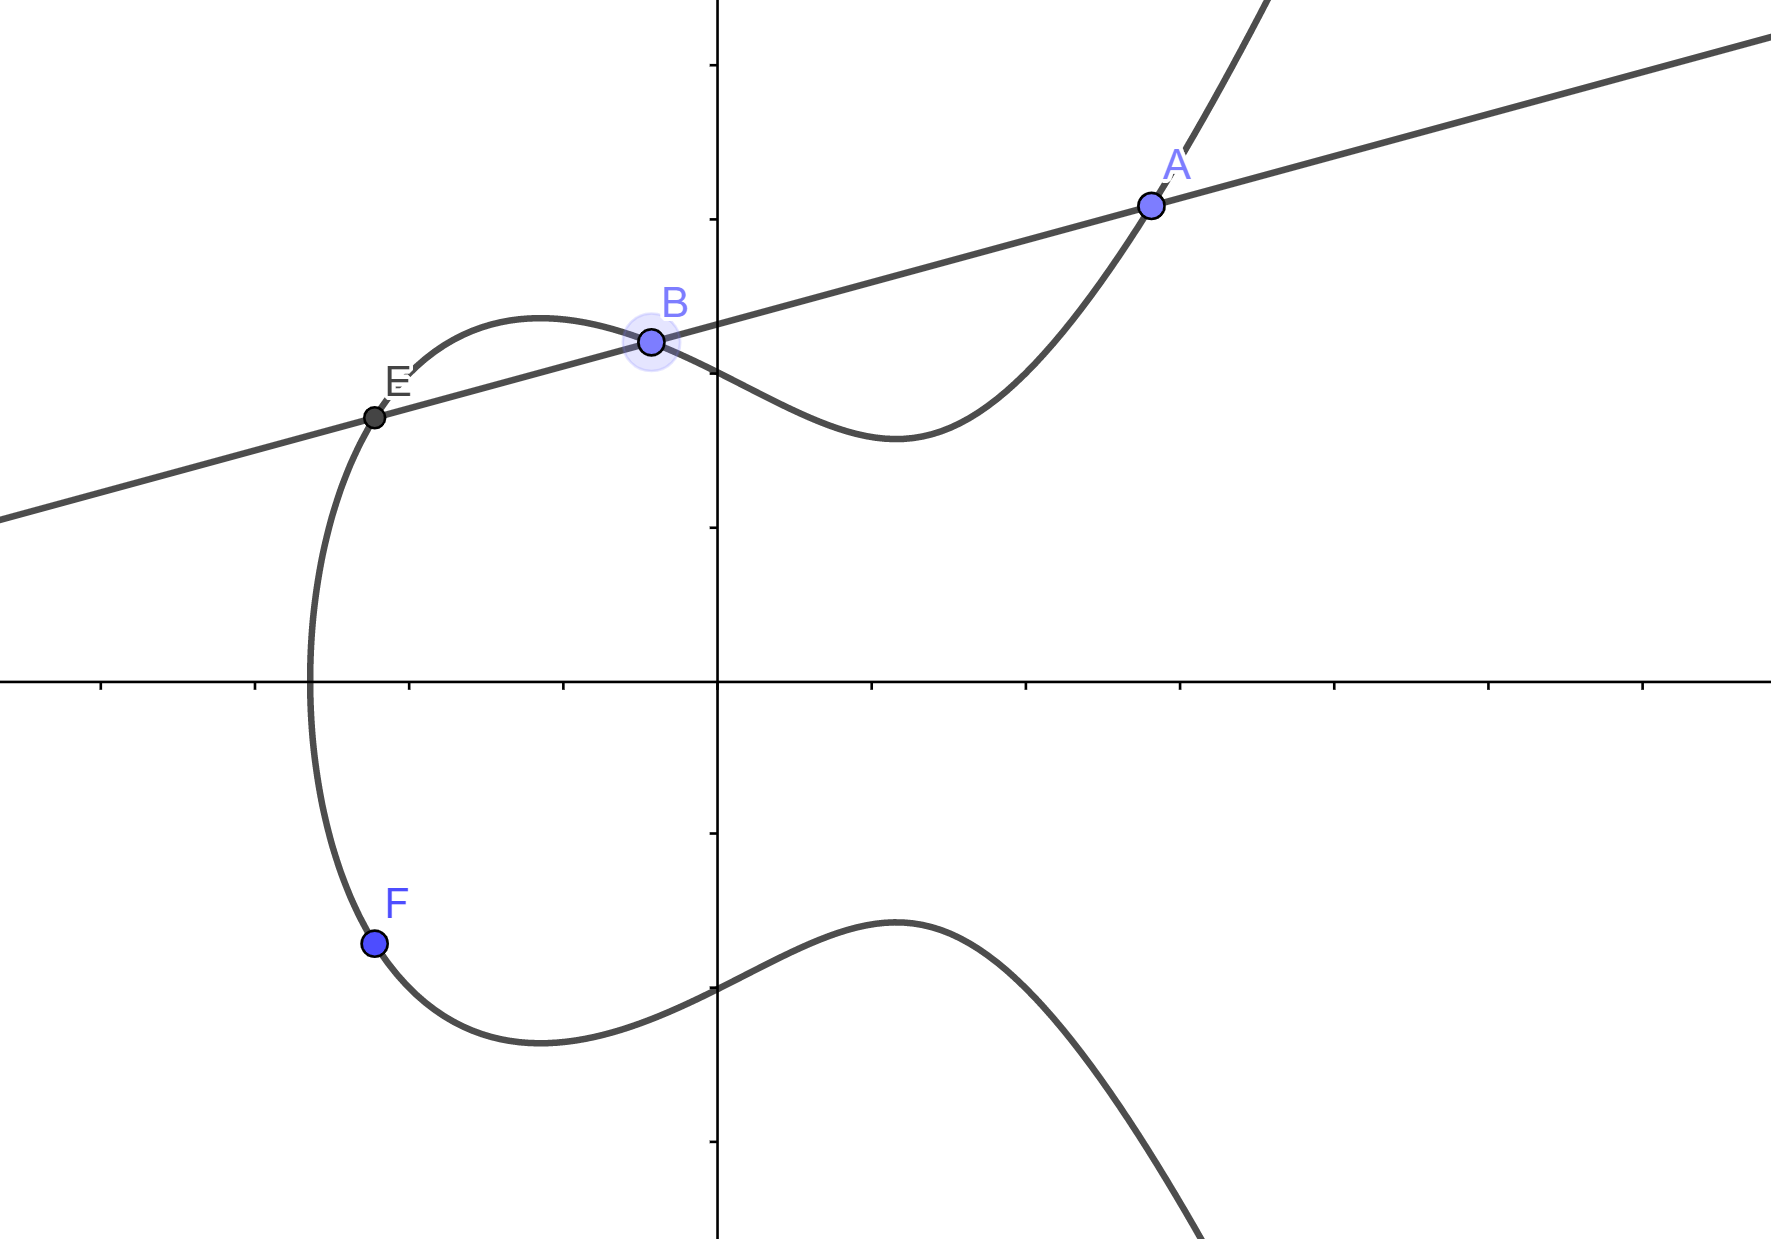
\includegraphics[width=15cm]{graphics/ec_summation.png}
\end{figure}
\begin{figure}[!h]
\caption{Иллюстрация операции удвоения на эллиптических кривых.}\label{fig:ec_doub}
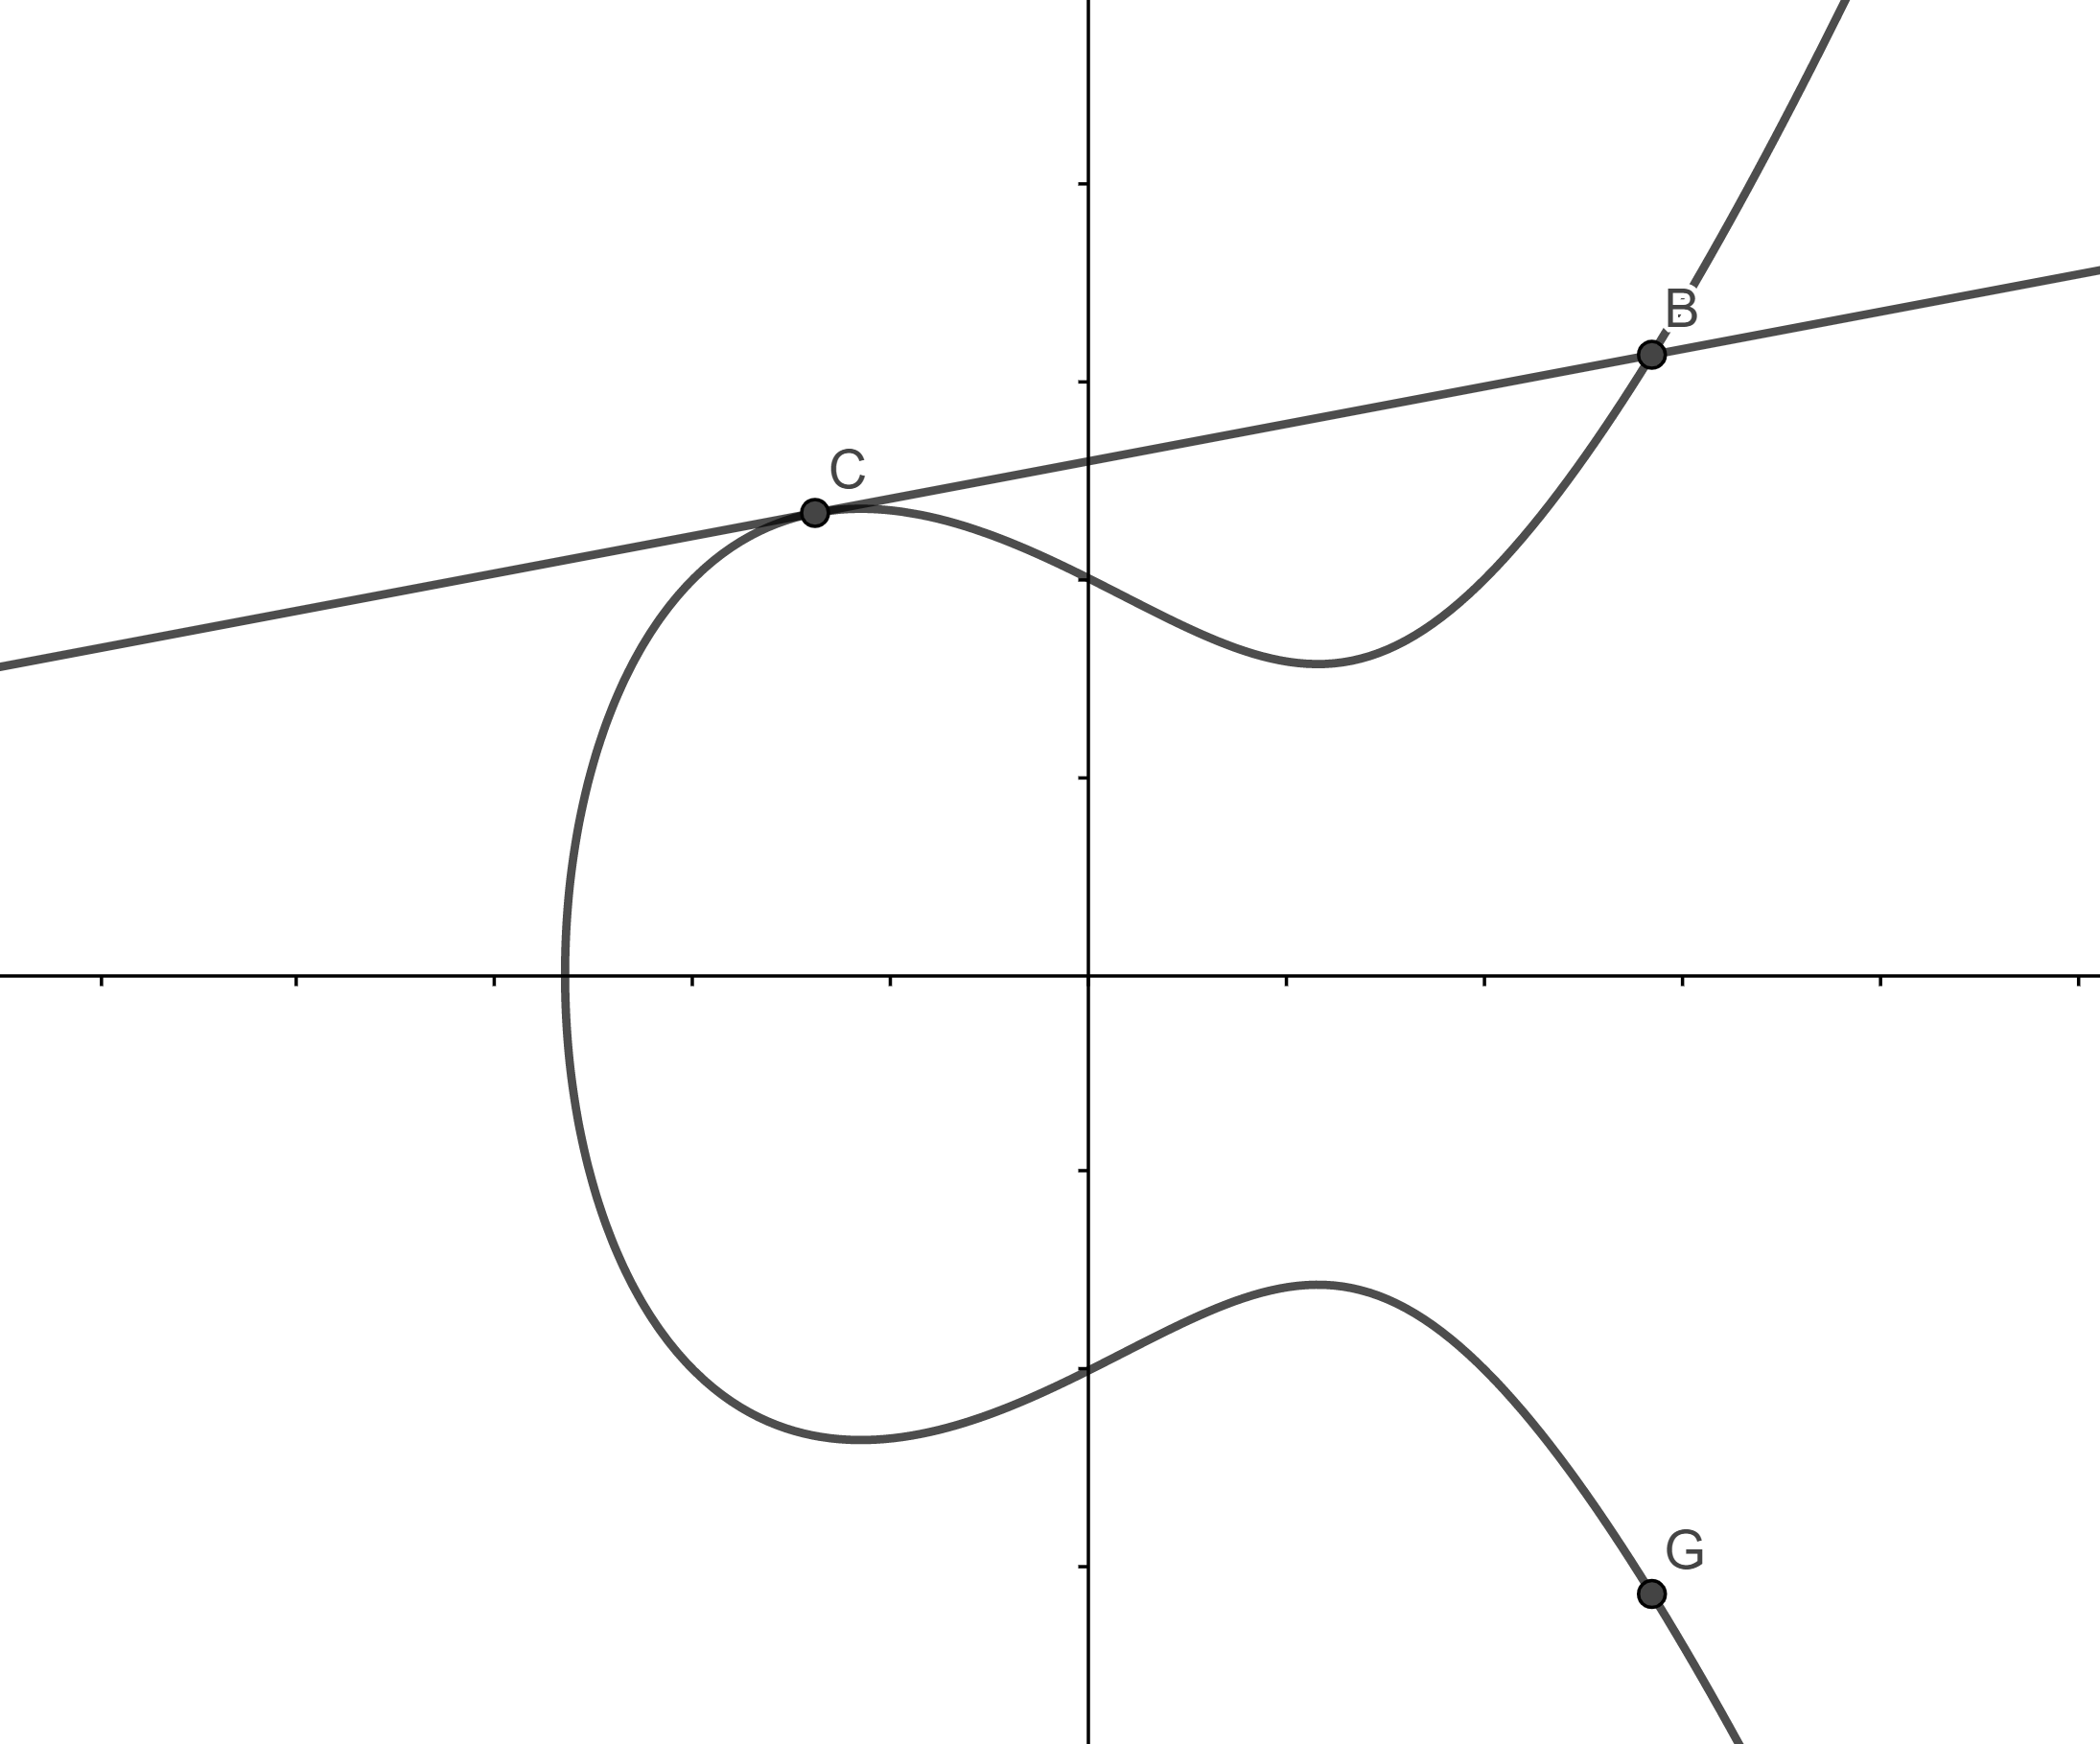
\includegraphics[width=15cm]{graphics/ec_doubling.png}
\end{figure}
Также в современной криптографии как односторонняя функция широко используется умножение на эллиптических кривых.
Эллиптическая кривая - это набор точек в конечном поле, подходящих под уравнение $y^2=x^3+ax+b$.
Умножение определено как повторяющееся $n$ раз сложение точки $P=(x,y)$, лежащей на этой кривой: $nP=P+P+\dots+P$
Сложение на эллиптической кривой можно описать как проведение линии через две точки, а затем отражение точки пересечения этой линии с кривой.
Если посмотреть на рисунок~\ref{fig:ec_sum}, то $A+B=-E=F$.
Для ускорения умножения можно использовать операцию удвоения, которую можно описать как проведение касательной к точке и
отражение точки пересечения касательной и кривой.
Если посмотреть на рисунок~\ref{fig:ec_doub}, то $C+C=-B=G$.
За счёт удвоения можно сократить количество операций с $n$ умножений до $log_2 n$ удвоений и небольшого числа умножений.
Это аналогично методу оптимизации <<возводи в квадрат и умножай>> для возведения числа в степень, который будет раскрыт в главе~\ref{sec:exp}.
На эллиптических кривых задача, обратная к умножению, также называется задачей дискретного логарифмирования.
Но на эллиптических кривых она решается за экспоненциальное время, то есть она сложнее, чем аналогичная задача на конечных полях.
За счёт этого в криптографии на эллиптических кривых используются ключи гораздо меньшего размера для достижения той же вычислительной сложности.\par
Несмотря на это, из-за сложностей реализации криптографии на эллиптических кривых чаще используется криптография в конечных полях.
Поэтому в данной работе рассматривается оптимизация алгоритма Диффи-Хэлмана именно для конечных полей $GF(2^k)$, которые подробно рассмотрены в главе~\ref{sec:fields}.


\section{Алгоритм Диффи-Хеллмана}\label{sec:dhke}

В 1976 году Уитфилдом Диффи и Мартином Хеллманом была опубликована статья <<New Directions in Cryptography>>
(<<Новые направления в криптографии>>)~\cite{dif77}, в которой были изложены основы криптографии с открытым ключом.
В отличие от симметричной криптографии, в которой ключ шифрования один и всегда держится в секрете,
в асимметричной криптографии у каждого пользователя существует два различных ключа - открытый (публичный) и закрытый (секретный).
Сообщение, зашифрованное открытым ключом, может быть расшифровано только соответствующим ему закрытым ключом, и наоборот.
Асимметричная криптография используется для широкого круга задач - от непосредственно шифрования до цифровых подписей.
Однако для шифрования коммуникаций целиком оно используется редко, так как асимметричное шифрование гораздо
медленнее симметричного.
Гораздо чаще с помощью асимметричного алгоритма устанавливается ключ, который используется для симметричного шифрования
последующих коммуникаций.
Именно для этой цели и предназначен алгоритм Диффи-Хеллмана.\par
Алгоритм Диффи-Хеллмана позволяет двум абонентам установить ключ для шифрования последующих коммуникаций,
используя только коммуникации по открытому каналу.
Это выгодно отличает его от предыдущих способов установления ключа шифрования, которые требовали передачи
физического ключа курьером или заказным письмом.
Алгоритм Диффи-Хеллмана основывается на задаче дискретного логарифмирования, и при правильном подборе условий,
взлом его требует решения задачи с суб-экспоненциальной или экспоненциальной временной сложностью.\par
Для непосредственного установления ключа два абонента \textbf{А} и \textbf{Б} должны выбрать базу $g$ и модуль $n$, которые
могут передаваться в открытом виде, и секретные ключи $a$ и $b$, которые генерируются случайно.
Каждый абонент независимо вычисляет открытые ключи:
\begin{gather*}
    A = g^a\pmod{n}\\
    B = g^b\pmod{n}\\
\end{gather*}
И пересылает их другому абоненту по незащищённому каналу связи.
Затем абоненты вычисляют секретный ключ:
\begin{gather*}
    S = A^b\pmod{n}\\
    S = B^a\pmod{n}\\
\end{gather*}
Который получается у них одинаковым из-за коммутативности показателей при последовательном возведении в степень:
\[(g^a)^b \pmod{n} \equiv (g^b)^a \pmod{n} \equiv g^{a*b}\pmod{n}\]
Полученный ключ $S$ можно использовать для последующего шифрования.
Если все коммуникации абонентов перехватят, то для получения ключа шифрования необходимо будет решить
вычислительную задачу Диффи-Хеллмана: найти $g^{ab}\pmod{n}$ по известным $g$, $n$, $g^a$ и $g^b$.
Решение задачи Диффи-Хеллмана можно свести к решению задачи дискретного логарифмирования~\cite{sma15},
для которой пока не известно решений за полиномиальное время.

У алгоритма Диффи-Хеллмана есть ещё одно важное преимущество, так как пары открытый-закрытый ключ ($a, g^a$) у каждого абонента независимы, любой абонент может инициировать
обновление общего секретного ключа.
С ростом объёма зашифрованных симметричным шифром данных повышается вероятность успешного подбора ключа с помощью
частотного криптоанализа.
Алгоритм Диффи-Хеллмана позволяет избежать этого установлением определённого периода времени или объёма данных
между обновлениями ключа симметричного шифрования.
Если использовать эту меру, даже после утечки ключа симметричного шифрования нарушитель получит доступ только к части
данных, но не ко всей переписке.

Для надёжности алгоритма необходимо правильно подбирать публичные переменные $g$ и $n$.
$n$ должно быть простым, но не все простые числа подходят для этого значения.
Например, если $n-1$ раскладывается на небольшие простые множители, задача дискретного логарифмирования
может быть решена за полиномиальное время с помощью алгоритма Полига-Хеллмана~\cite{men01}.
Поэтому большинство имплементаций следуют рекомендациям IETF (инженерного совета Интернета)~\cite{rfc7296}, в которых
приводятся рекомендуемые значения переменных $g$ и $n$.

Повсеместное следование рекомендациям IETF в сочетании с требованиями правительства США к экспортной криптографии
привело к тому, что некоторые сервера можно заставить использовать устаревшие стандарты криптографии, в которых
используется небольшой размер ключа менее 512 бит~\cite{adr15}.
Существуют алгоритмы, позволяющие с помощью предварительных вычислений сократить время решения задачи
дискретного логарифмирования для известного из рекомендаций значения $n$ длиной 512 бит до примерно 70 секунд, что сводит
безопасность шифрования к нулю.
В той же статье было высказано предположение, что ключи в 768 бит также небезопасны, а ключи длиной
в 1024 бит могут быть скомпроментированы с ресурсами правительства и не должны считаться достаточными для шифрования.
Таким образом, для достижения безопасности коммуникаций рекомендуется использовать ключи длиной от 2048 бит,
для которых задача дискретного логарифмирования в $10^9$ раз сложнее, чем для 1024 бит.

Но с использованием более длинных ключей растёт и время работы алгоритма.
Основные вычисления в алгоритме Диффи-Хеллмана - это возведения в степень по модулю, используемые для вычисления секретных ключей,
которые выполняются за полиномиальное время.
Но алгоритм можно оптимизировать и внутри этого класса временной сложности.
С помощью оптимизации алгоритма, которая рассматривается в данной работе, можно достичь удлинения ключей шифрования
практически в полтора раза по сравнению со стандартной реализацией без потерь в скорости работы.
То есть реализации, которые использовали ключи в 1024 бита, смогут перейти на ключи в 1536 бит без потерь в скорости работы,
но с экспоненциальным приростом временной сложности задачи дискретного логарифмирования, и, следовательно, безопасности
шифрования.

\section{Конечные поля}\label{sec:fields}

Современная криптография с открытым ключом основана на арифметике остатков~\cite{sma15, men01, knu97_2}.
В арифметике остатков для любых вычислений фиксируется положительное натуральное число $N$, которое называется модулем.
Если разность двух чисел $b-a$ делится нацело на $N$, то $a$ и $b$ сравнимы по модулю $N$:
\[a \equiv b \pmod{N}\]
В этом случае $a$ и $b$ имеют одинаковый остаток от деления на $N$.
Все возможные остатки от деления чисел на $N$ образуют множество значений оператора модуля $\pmod{N}$:
\[\mathbb{Z}/N\mathbb{Z}=\{0,\dots,N-1\}\]
Поскольку все сравнимые по между собой по модулю $N$ числа имеют один и тот же остаток, можно считать, что
элемент $x\in\mathbb{Z}/N\mathbb{Z}$ - это представление класса чисел вида $x+kN, k\in\mathbb{Z}$.
Таким образом, при операциях по модулю $N$ можно считать сравнимые между собой числа равными друг другу:
\[a+kN\pmod{N} = a, k \in \mathbb{Z}\]


На множестве $\mathbb{Z}/N\mathbb{Z}$ определены две основных операции -- сложение и умножение.
Они определяются через аналогичные операции на множестве целых чисел.
Они обладают следующими свойствами:
\begin{enumerate}[label=\arabic*.]
    \item Замкнутость сложения и умножения:
    \[\forall a, b \in \mathbb{Z}/N\mathbb{Z}: a+b\in \mathbb{Z}/N\mathbb{Z}, a*b\in \mathbb{Z}/N\mathbb{Z}\]
    \item Ассоциативность сложения и умножения:
    \[\forall a, b, c \in \mathbb{Z}/N\mathbb{Z}: (a+b)+c = a+(b+c), (a*b)*c = a*(b*c)\]
    \item Существование единичного элемента по сложению и умножению:
    \[\forall a \in \mathbb{Z}/N\mathbb{Z}: a+0 = 0+a = a, a*1 = 1*a = a\]
    \item Существование обратного элемента по сложению:
    \[\forall a \in \mathbb{Z}/N\mathbb{Z}: a+(N-a) = (N-a)+a = 0\]
    \item Коммутативность сложения и умножения:
    \[\forall a, b \in \mathbb{Z}/N\mathbb{Z}: a+b = b+a, a*b = b*a\]
    \item Сложение и умножение связаны законом дистрибутивности:
    \[\forall a, b, c \in \mathbb{Z}/N\mathbb{Z}: (a+b)*c = a*c + b*c\]
\end{enumerate}
Множество, на котором определена операция, удовлетворяющая свойствам $1-4$, называется группой.
Если эта операция удовлетворяет и свойству $5$, она называется коммутативной.
Группы классифицируются по типу групповой операции - аддитивные $(G, +)$ и мультипликативные $(G,*)$.
Группа, в которой существует элемент, многократным применением к которому групповой операции можно получить
любой другой элемент этой группы, называется циклической, а такой элемент -- образующей.
Например, в группе целых чисел по сложению образующей будет $1$.

Образующая $g$ для циклической группы $G$ обозначается $G=\langle g \rangle$.
В мультипликативном случае каждый элемент $h$ группы $G$ можно записать как:
\[\forall h \in G: h=g^x\]
А в аддитивном случае:
\[\forall h \in G: h=g*x\]
$x$ в обоих случаях -- некоторое целое число, называемое дискретным логарифмом $h$ по основанию $g$.

Множество $R$, на котором определены две операции -- сложение и умножение, которые обладают свойствами
$1-5$, кроме коммутативности умножения, называется кольцом $(R,*,+)$.
Если операция умножения в данном кольце коммутативна, оно называется коммутативным кольцом.
Приведённое выше множество остатков $\mathbb{Z}/N\mathbb{Z}$ с операциями сложения и умножения
является коммутативным кольцом и называется кольцом вычетов по модулю $N$.

Одна из главных задач арифметики остатков -- это поиск элемента $x\in\mathbb{Z}/N\mathbb{Z}$, который удовлетворяет равенству:
\[a*x=b\pmod{N}\]
С вещественными коэффициентами при $a \neq 0$ линейное уравнение $a*x=b$ всегда разрешимо.
При рассмотрении над кольцом целых чисел не всегда существует ответ, а для кольца вычетов есть три случая,
которые разделяются в зависимости от наибольшего общего делителя (НОД) чисел $a$ и $N$.
\begin{enumerate}[label=\arabic*.]
    \item Уравнение может иметь ровно одно решение при НОД$(a,N) = 1$:
    \[2*x=3\pmod{91}\]
    \item Может иметь $g = $ НОД$(a,N)$ решений при $g \neq 1$ и $b$, делимом на $g$:
    \[3*x=6\pmod{91}\]
    \item В других случаях уравнение решений не имеет:
    \[7*x=3\pmod{91}\]
\end{enumerate}

При НОД$(a,N) = 1$ числа $a$ и $N$ называются взаимно простыми.
Число элементов кольца $\mathbb{Z}/N\mathbb{Z}$, взаимно простых с $N$, можно найти с помощью функции Эйлера \varphi.
$\varphi(N)$ можно найти с помощью разложения $N$ на простые множители.
Если $p_i$ - различные простые числа:
\begin{gather*}
    N = \prod_{i=1}^n p_i^{e^i}\\
    \varphi(N) = \prod_{i=1}^n p_i^{e^i-1}(p_i-1)\\
\end{gather*}
Следовательно, для простого $p$:
\[\varphi(p) = p-1\]
И для простых $p$ и $q$, $p \neq q$:
\[\varphi(p*q) = (p-1)*(q-1)\]
Для взаимно простых $a$ и $N$ существует единственное $c$, удовлетворяющее следующему равенству:
\[a*c \equiv c*a \equiv 1 \rmod{N}\]
Это $c$ называется мультипликативным обратным к $a$ и обозначается как $a^{-1} \pmod{N}$.
При простом модуле $N=p$ для любого ненулевого элемента $N$ существует единственно мультипликативно обратное.
\[ \forall a \in (\mathbb{Z}/p\mathbb{Z}) \backslash \{0\} ~ \exists! a^{-1}: a*a^{-1} = 1 \pmod{p}\]

Коммутативное кольцо $(F,*,+)$, которое также обладает следующими свойствами:
\begin{enumerate}[label=\arabic*.]
    \item $(F,+)$ -- коммутативная группа с единичным элементом 0,
    \item $(F \backslash \{0\},*)$ -- коммутативная группа с единичным элементом 1,
    \item $0\neq1$ -- единичные элементы по сложению и умножению неравны,
    \item $(F,*,+)$ -- операции сложения и умножения удовлетворяют закону дистрибутивности.
\end{enumerate}
Называется конечным полем.
Конечное поле - это коммутативное кольцо, в котором каждый элемент обратим.
Если $(\mathbb{Z}/N\mathbb{Z})^*$ -- множество обратимых элементов в $\mathbb{Z}/N\mathbb{Z}$:
\[(\mathbb{Z}/N\mathbb{Z})* = \{x \in \mathbb{Z}/N\mathbb{Z} | ~ \text{НОД}(x, N) = 1\}\]
Количество элементов этого множества будет равно значению функции Эйлера:
$|(\mathbb{Z}/N\mathbb{Z})^*| = \varphi (N)$.

При простом $N=p$ каждый элемент кольца $\mathbb{Z}/p\mathbb{Z}$ взаимно прост с $p$ и поэтому обратим.
Из этого следует два свойства:
\begin{gather*}
    (\mathbb{Z}/p\mathbb{Z})^* = \{1, \dots, p-1\}\\
    F \backslash \{0\} = F^*\\
\end{gather*}
Целые числа по модулю $N$ образуют поле тогда и только тогда, когда $N$ -- простое число.

Конечные поля существуют не только на целых числах.
В криптографии используется более общий тип конечных полей, на которых могут быть переопределены операции сложения и умножения.
Основанием такого поля является простое число $p$ в степени $k$.
В данной работе рассматриваются поля $GF (2^k)$, содержащие $2^k$ элементов.
Переменные в таких полях можно представлять как многочлены от степеней основания поля:
\[a(x) \in GF(2^k) = \sum_{i=0}^{k-1}a_i x^i = a_{k-1}x^{k-1} + a_{k-2}x^{k-2} + \dots + a_1 x + a_0\]
Уравнение для целых чисел по модулю $N$:
\[a*x = b \pmod{N}\]
Для конечных полей $GF(2^k)$ переопределяется как:
\[a(x) \cdot \alpha = b(x) \pmod{f(x)}]\]
Как и в случае для целых чисел, ответ зависит от НОД$(a(x), f(x))$.
Многочлен называется неприводимым, если у него нет делителей, отличных от него самого и единичного элемента.
Таким образом, неприводимые многочлены являются аналогами простых чисел в конечных полях.
Конечное поле всегда определено относительно неприводимого многочлена.

% Здесь можно расписать про изоморфизм. Нужно ли?
Для любых двух конечных полей с одинаковым основанием (степенью простого числа), определённых относительно различных
неприводимых многочленов можно построить однозначное отображение всех элементов одного поля в другое.
То есть для любого основания существует единственное (с точностью до изоморфизма) конечное поле с числом
элементов, равным степени простого числа.
Ненулевые элементы конечного поля $GF(2^k)^*$ составляют конечную коммутативную циклическую группу.
Образующая группы $GF(2^k)^*$ называется примитивным элементом конечного поля.
Примитивный элемент существует в любом конечном поле, и любой ненулевой элемент поля может быть выражен через его степень:
\[\forall \alpha \in GF(2^k)^* ~ \exists x \in \mathbb{Z}: \alpha = g^x\]

Теперь можно разъяснить, что для реализации алгоритма Диффи-Хеллмана на конечных полях открытые параметры алгоритма
$g$ и $n$ -- переопределяются соответственно как примитивный элемент и неприводимый многочлен, определяющие конечное поле.
Переменные же $a$ и $b$ -- элементы этого конечного поля.
Переопределение операций умножения и возведения в степень раскрыто в главах~\ref{sec:oper} и~\ref{sec:exp}.

Конечные поля $GF(2^k)$ широко применяются в криптографии.
Основная причина для широкого использования - это простота в имплементации и скорость работы.
Эти показатели достигаются за счёт структуры памяти ЭВМ.
В бинарной структуре (true/false) ячеек памяти ЭВМ можно без каких-либо модификаций хранить элементы
таких полей, а также возможны различные оптимизации операций сложения и умножения.
Эти преимущества распространяются и на программные, и на физические имплементации~\cite{koc98}.
Для сравнения, имплементации полей на $GF(p^k)$ для $p > 2$ сложнее, и аналогичные операции в таких полях выполняются
примерно в два раза медленнее~\cite{mau15}.


\section{Некоторые операции в конечных полях}\label{sec:oper}

% Эта глава и все последующие будут раскрыты подробнее после предзащиты
В конечных полях $GF(2^k)$ операции сложения и вычитания переопределены как сложение по модулю $2$.
Эта операция похожа на сложение в двоичной системе, но переполнения модуля отбрасываются, то есть нет переносов.
То есть в конечном поле $GF(2^k)$ $1+1 = 1-1 = 0$.
На ЭВМ эта операция реализуется через побитовое исключающее ИЛИ и выполняется эффективно - специальной инструкцией процессора.

Умножение производится относительно неприводимого многочлена $n(x)$:
\[c(x) = a(x) \cdot b(x)\pmod{n(x)}\]
и все переносы также отбрасываются.
Умножение и деление на два  на ЭВМ производятся через побитовые сдвиги:
\[a(x) \cdot x = \sum_{i=0}^{k-1}a_i x^i = a_{k-2}x^{k} + a_{k-2}x^{k-1} + \dots + a_1 x^2 + a_0 x\]
После умножения на 2 для взятия модуля может быть вычтен неприводимый многочлен.

В реализации для данной работы для умножения использовался модифицированный метод "древнеегипетского" или "крестьянского"
умножения.
Для данных $a(x)$ и $b(x)$ алгоритм получает $c(x) = a(x) \cdot b(x) \pmod{n(x)}$:
\begin{enumerate}[label=\arabic*:]
    \item $c(x)=0$
    \item for i=0 to k-1
    \item \hspace*{10mm} $c(x) = c(x) + b_0 a(x)$
    \item \hspace*{10mm} $b(x) = b(x)/x$
    \item \hspace*{10mm} $car = a_{k-1}$
    \item \hspace*{10mm} $a(x) = a(x) \cdot x$
    \item \hspace*{10mm} if $car == 1$: $a(x) = a(x) - n(x)$
\end{enumerate}
Если на каком-то шаге значение $a(x)$ становится больше неприводимого многочлена (что выявляется на шаге 5), на шаге 7
от него берётся остаток по модулю.
Отметим, что это происходит через эффективную операцию побитового исключающего или.
Сумма двух элементов $GF(2^k)$ никогда не будет больше неприводимого многочлена, так как переносы при сумме отбрасываются.
Следовательно, на четвёртом шаге алгоритма операция взятия остатка по модулю не нужна.

Для вычисления НОД и мультипликативно обратного использовалась вариация расширенного алгоритма Евклида
- алгоритм Бланкиншипа.
Вычисляется $a(x) \cdot u + n(x) \cdot v =$ НОД$(a(x), n(x)) = 1$.
$u$ будет мультипликативно обратным к $a(x)$.
В алгоритме Бланкиншипа определяется матрица:
\begin{equation*}
M =
\begin{pmatrix}
a(x) & 1 & 0 \\
b(x) & 0 & 1\\
\end{pmatrix}
\end{equation*}
Затем к первому столбцу применяется расширенный алгоритм Евклида, распространяя операции на остальные.
Алгоритм заканчивается, когда в первом столбце появляется НОД$(a(x), b(x))$.
Во второй строке остаются $1, u, v$.

Для возведения в степень в конечных полях используются различные алгоритмы бинарного возведения в степень.
В данной работе используется самый распространённый алгоритм возведения в степень слева направо\\
(left-to-right binary exponentiation)~\cite{koc97}.
Для данных $m(x)$ и $e$ алгоритм позволяет вычислить $c(x) = m(x)^e \pmod{n(x)}$ в разы быстрее метода последовательных умножений:
\begin{enumerate}[label=\arabic*:]
    \item $c(x) = 1$
    \item for i=k-1 downto 0
    \item \hspace*{10mm} $c(x) = c(x)\cdot c(x)$
    \item \hspace*{10mm} if $e_i$ == 1: $c(x) = m(x) \cdot c(x)$
\end{enumerate}
Умножения в алгоритме выполняются по вышеуказанному модифицированному крестьянскому алгоритму и учитывают остатки от деления.

Имплементация данных операций позволила получить эффективную реализацию алгебры в конечных полях $GF(2^k)$.
Эта реализация аналогична существующим аналогам, которые лежат в основе многих стандартных криптографических библиотек.
Она служила опорной точкой для сравнения с оптимизированными вариантами, которые описаны далее.


\section{Алгоритм Монтгомери}\label{sec:mont}

Здесь будет описание алгоритма и формы Монтгомери, а также принципы, благодаря которым этот способ быстрее.
Также будет представлено описание адаптации алгоритма на клеточные автоматы, с помощью которой
возможна реализация на
Источниками будут~\cite{jeo07, men01, koc97}.

\section{Клеточные автоматы}\label{sec:cells}

В этой главе будет рассказано о клеточных автоматах, их истории и структуре.
Также будет рассказано об их применениях в криптографии.
Как источники будут использоваться~\cite{zhu17, zhu17_2}.

\section{Параллелизация алгоритма Монтгомери}\label{sec:paramont}

Здесь будет пересказ статьи~\cite{ku04} с подробным описанием алгоритма.
Также будет объяснение перевода алгоритма на клеточные автоматы.
Клеточные автоматы в рамках данной работы - это абстракция, позволяющия объяснить алгоритм.
Но эта абстракция ценна тем, что с её использованием можно создать реализацию "в железе" с логическими элементами.

\finishrelatedwork
\chapterconclusion

Будут подведены итоги, объяснён выбор конкретных алгоритмов (основной использующийся, стандартный
Монтгомери и параллелизация Монтгомери) и приведены теоретические прогнозы по приросту производительности
из источников.

\chapter{Имплементация и тестирование}

\section{Выбор языка программирования}\label{sec:prog}

Будет рассказано про особенности языка Python, за которые он был выбран для данного проекта.
В частности, про то, что в Python переменные и числа не имеют ограничения по длинне, что делает
возможным тестирование на очень длинных ключах.
Также будут описаны альтернативы (performance-focused implementations из статьи) и их недостатки.

\section{Описание имплементации}\label{sec:impl}

Здесь будет не очень много, в основном структура и ссылки на алгоритмы из первой главы.
В приложении будет код - не весь, но некоторых функций.
Возможно, будут ссылки на упомянутые ранее альтернативы:~\cite{pri16, mau15}

\section{Методология тестирования производительности}\label{sec:meth}

Ссылки на наборы многочленов~\cite{rfc7296, rfc3526} и повторный рассказ о методиках их выбора~\cite{rfc2412}.
Также упор на многократное тестирование на случайных числах.
Тут в основном, опять же, из статьи.

\section{Результаты тестирования производительности}\label{sec:results}

Графики из статьи на русском и их описание.

\chapterconclusion

Подробный разбор результатов тестирования с акцентом на приросте в производительности почти в полтора раза.

\startconclusionpage

Краткое описание достигнутых результатов, акцент на возможности реализации "в железе"
и минимальности изменений для программной.
Также акцент на том, что прирост в производительности универсален и может быть применён не только для Диффи-Хеллмана
и в теории для эллиптических кривых~\cite{sta03} как further research.

\printmainbibliography


\appendix

\chapter{Секции исходного кода имплементации}\label{sec:app:1}

    Некоторые критические функции и ссылка на репозиторий.

\end{document}
